\documentclass[letterpaper]{article}
\usepackage[utf8]{inputenc}
\usepackage[T1]{fontenc}
\usepackage[activeacute,english]{babel}
\usepackage[vmargin=4cm,tmargin=3cm,hmargin=2cm,letterpaper]{geometry}%
\usepackage{helvet}
\usepackage{amsmath,amsfonts,amssymb}
\usepackage{graphicx}
\usepackage{color}
\usepackage{xcolor}
\usepackage{verbatim}
\usepackage{tabls}
\usepackage{lastpage}
\usepackage{fancyhdr}
\usepackage{url}
\usepackage{listings}
\usepackage{tikz}
\usepackage{pgf}
\usepackage{pgffor}
\usepgfmodule{plot}
\usepackage{wrapfig}
\usepackage{ifpdf}
\usepackage{amssymb}
\usepackage{pifont}
\usepackage{epstopdf}
\usepackage{graphicx} % Allows including images
\usepackage{booktabs} % Allows the use of \toprule, \midrule and \bottomrule in tables
\usepackage{tikz}
\usetikzlibrary{arrows,decorations,snakes,backgrounds,fit,calc,through,scopes,positioning,automata,chains,er,fadings,calendar,matrix,mindmap,folding,patterns,petri,plothandlers,plotmarks,shadows,shapes,shapes.arrows,topaths,trees}

\lstset{% general command to set parameter(s)
%   basicstyle=\small,
  % print whole listing small
%   keywordstyle=\color{black}\bfseries\underbar,
  % underlined bold black keywords
%   identifierstyle=,
  % nothing happens
%   commentstyle=\color{white}, % white comments
%   stringstyle=\ttfamily,
  % typewriter type for strings
  showstringspaces=false}
  % no special string spaces

\pagestyle{fancy}
\color{black}
\fancyhead{}
\renewcommand{\headrule}{\hrule\vspace*{0.5mm}\rule{\linewidth}{0.8mm}}
\renewcommand{\familydefault}{\sfdefault}

\graphicspath{{./images/}}
\lhead{
\includegraphics[width=2cm]{logoucr.png}}
\rhead{
\includegraphics[width=3cm]{eie-text-gray-6x3cm.png}}
\chead{UNIVERSIDAD DE COSTA RICA\\FACULTAD DE INGENIERÍA\\ESCUELA DE INGENIERÍA ELÉCTRICA\\\textbf{ESTRUCTURAS ABSTRACTAS DE DATOS Y\\ ALGORITMOS PARA INGENIERÍA}\\IE-0217\\I CICLO 2014\\PROPUESTA DE PROYECTO ESTRUCTURAS DE DATOS}

\lfoot{}%
\cfoot{}%
%\cfoot{\thepage\ de \pageref{LastPage}}%
\rfoot{}%

%%%%%%%%%%%%%%%%%%%%%%%%%%%%%%%%%%%%%%%%%%%%%%%%%%%%%%%%%%%%%%%%%%%%%%%%%%%%%%%%%%%%%%%%%%%%%%%%%%%%%%%%%%%%%%%
\newcommand{\uic}{blue} %user-input color
%%%%%%%%%%%%%%%%%%%%%%%%%%%%%%%%%%%%%%%%%%%%%%%%%%%%%%%%%%%%%%%%%%%%%%%%%%%%%%%%%%%%%%%%%%%%%%%%%%%%%%%%%%%%%%%%%%
\newcommand{\uim}{\_\_} %user-input marker
%%%%%%%%%%%%%%%%%%%%%%%%%%%%%%%%%%%%%%%%%%%%%%%%%%%%%%%%%%%%%%%%%%%%%%%%%%%%%%%%%%%%%%%%%%%%%%%%%%%%%%%%%%%%%%%%%%
\newcommand{\userinput}[1]{\textcolor{\uic}{\uim#1\uim}}


%%%%%%%%%%%%%%%%%%%%%%%%%%%%%%%%%%%%%%%%%%%%%%%%%%%%%%%%%%%%%%%%%%%%%%%%%%%%%%%%%%%%%%%%%%%%%%%%%%%%%%%%%%%%%%%%%%
\begin{document}\vspace*{2cm}
%%%%%%%%%%%%%%%%%%%%%%%%%%%%%%%%%%%%%%%%%%%%%%%%%%%%%%%%%%%%%%%%%%%%%%%%%%%%%%%%%%%%%%%%%%%%%%%%%%%%%%%%%%%%%%%%%%

%%%%%%%%%%%%%%%%%%%%%%%%%%%%%%%%%%%%%%%%%%%%%%%%%%%%%%%%%%%%%%%%%%%%%%%%%%%%%%%%%%%%%%%%%%%%%%%%%%%%%%%%%%%%%%%%%%
\begin{center}
\Huge
\textbf{Kinect Data Library}
\vspace*{1cm}
\end{center}

\noindent
\small\baselineskip=14pt
\textbf{Estudiantes:} \\
\text{David Pérez Bolaños - B04769}\\
\text{Andrey Pérez Salazar - B25084}\\
\text{Andrés Sánchez López - B26214}\\


%\begin{figure}[ht]
%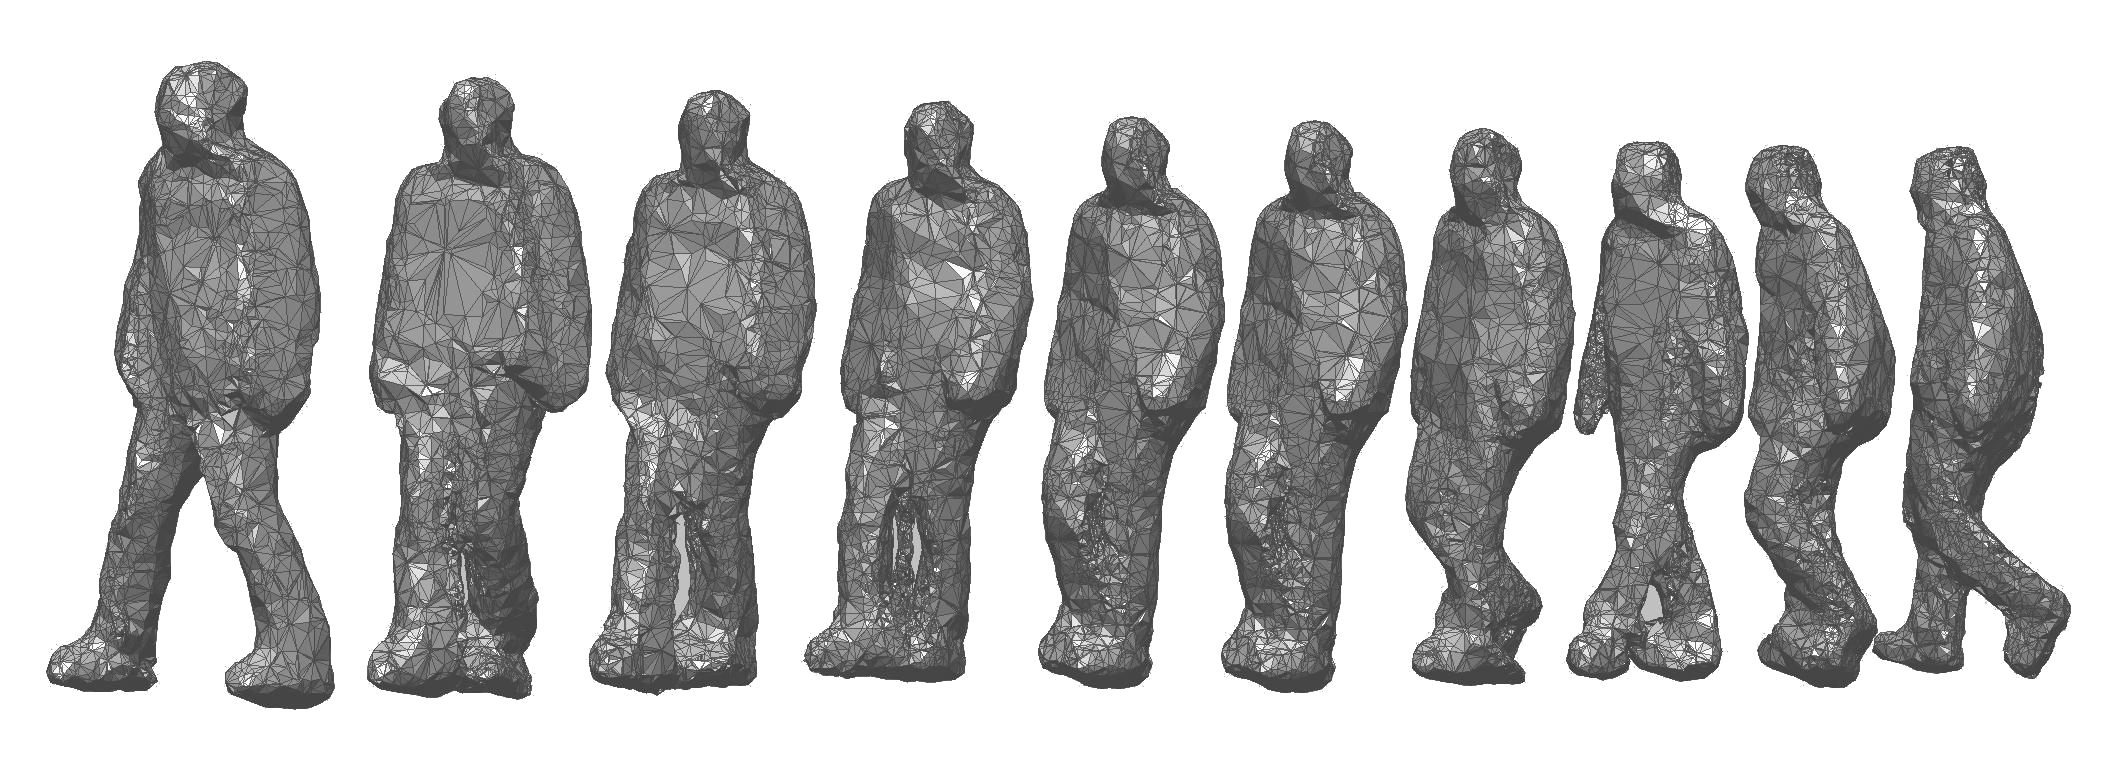
\includegraphics[width=1\linewidth]{visual_hull_4.png}
%\end{figure}


%%%%%%%%%%%%%%%%%%%%%%%%%%%%%%%%%%%%%%%%%%%%%%%%%%%%%%%%%%%%%%%%%%%%%%%%%%%%%%%%%%%%%%%%%%%%%%%%%%%%%%%%%%%%%%%%%%
\section{Introducción}
\hyphenation{fun-cio-na-li-dad}
Una estructura de datos es ... (No tengo idea)

%%%%%%%%%%%%%%%%%%%%%%%%%%%%%%%%%%%%%%%%%%%%%%%%%%%%%%%%%%%%%%%%%%%%%%%%%%%%%%%%%%%%%%%%%%%%%%%%%%%%%%%%%%%%%%%%%%
\section{Objetivos}

\subsection{Objetivo General}


El objetivo general consiste en .\\


\subsection{Objetivos Específicos}

Los objetivos específicos son:\\

\begin{enumerate}
\item Ampliar el conocimiento de. 
\item Desarrollar .
\item Obtener .
\end{enumerate}

%%%%%%%%%%%%%%%%%%%%%%%%%%%%%%%%%%%%%%%%%%%%%%%%%%%%%%%%%%%%%%%%%%%%%%%%%%%%%%%%%%%%%%%%%%%%%%%%%%%%%%%%%%%%%%%%%%
\section{Metodología}


Se realizará la investigación sobre librerías que se necesiten para la manipulación de objetos tridimensionales. Previamente, se revisarán las 
librerías encontradas, para determinar la necesidad de nuestro proyecto. 
Una vez hecho esto, se buscará implementar una librería en el lenguaje C++.\\

Lo que se realizará primero, es una investigación sobre que funciones presentan las librerías encontradas en lenguaje C++ y estudiar el código de estas,
esto con el fin de entender la utilización de los datos en estos códigos, todo esto, en caso de haber encontrado una librería en lenguaje C++ con relación a este tema.
Para lograr esto, se leerá toda la bibliografía necesaria para poder entender de la mejor manera que es lo que se necesita exactamente. Una vez
entendido algunas de las diferentes implementaciones ya existentes, se pretende crear una librería en lenguaje C++ con funciones de comparación entre datos
recibidos en diferentes momentos y así determinar mejorías o fallas. \\

Será necesario también, la utilización de un
kinect para obtener datos de diferentes figuras tridimensionales de tal modo que se pueda dar una revisión de la librería. Finalmente, se buscará ajustar tal librería,
de modo que sea fácil para el usuario la utilización de la misma, para que sea utilizada como una solución de las necesidades
existentes sobre objetos tridimensionales.\\

%%%%%%%%%%%%%%%%%%%%%%%%%%%%%%%%%%%%%%%%%%%%%%%%%%%%%%%%%%%%%%%%%%%%%%%%%%%%%%%%%%%%%%%%%%%%%%%%%%%%%%%%%%%%%%%%%%


\section{Cronograma}

\begin{center}
\begin{tabular}{l l   @{\hspace{1cm}}p{10cm}}
\cline{3-3}

\toprule
\textbf{Semana} & \textbf{Fechas} & \textbf{Actividad} \\
\midrule
1 & 28 de abril a 4 de mayo & Entrega de la propuesta - Instalación del
software para uso del kinect - Estudio del software para uso del kinect -
Estudio del lenguaje C++ \\
2 & 5 de mayo a 14 de mayo & Desarrollo, en lenguaje C++, de la función
de comparación. \\

3 & 15 de mayo a 17 de mayo & Prueba de la función utilizando datos
provenientes del kinect. \\
4 & 19 de mayo a 19 de mayo & Realización de la presentación e informe
escrito del proyecto. \\
\bottomrule
\end{tabular}
\end{center}

\begin{figure}[ht]
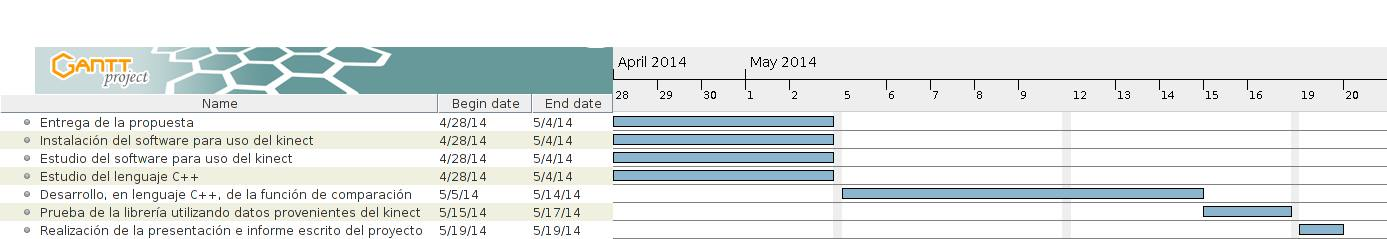
\includegraphics[width=1\linewidth]{10288526_791857134159417_2036565498_o.jpg}
\end{figure}

\section{Referencias}

\begin{enumerate}

\item Richard, J. Computer Science Division. University of California at Berkeley. Triangle. A Two-Dimensional Quality Mesh Generator and 
Delaunay Triangulator. Encontrado el 13 de abril del 2014 en: http://www.cs.cmu.edu/~quake/triangle.html
\item Escenografía Intermedial. Nuevos medios y tecnologías afines a la escena. (15 de mayo del 2012).
Nube de puntos (Point Cloud) con Kinect. Encontrado el 13 de abril del 2014 en: http://escenografiaaumentada.wordpress.com/2012/05/15/148/
\item OPENKINECT. Encontrado el 13 de abril del 2014 en: http://openkinect.org/wiki/Main\_Page

\end{enumerate}

	
\end{document}

